\documentclass[MPSI]{cours}

\begin{document}
\setcounter{chapter}{8}
\chapter{Propagation d'un signal, ondes}
\section{Définition}
Un onde correspond à la propagation d'une perturbation des propriétés physiques locales d'un milieu.
\section{Exemples d'ondes}
\begin{itemize}
\item acoustique (son) : Perturbation de la pression de l'air,\\
Vitesse de propagation : $\simeq \SI{340}{m/s}$ dans l'air, $\simeq \SI{1500}{m/s}$ dans l'eau, $\simeq \SI{5800}{m/s}$ dans l'acier. \\
fréquences caractéristiques : 
\begin{itemize}
\item \SI{20}{Hz}--\SI{20}{kHz} : audition humaine
\item Jusqu'à \SI{200}{kHz} : chauve-souris
\item \SI{2}{MHz}--\SI{3}{GHz} : échographie
\end{itemize}

\item électromagnétique : perturbation du champ électromagnétique (dans le vide)\\
vitesse de propagation : \SI{3e8}{m/s} dans le vide
fréquences caractéristiques : 

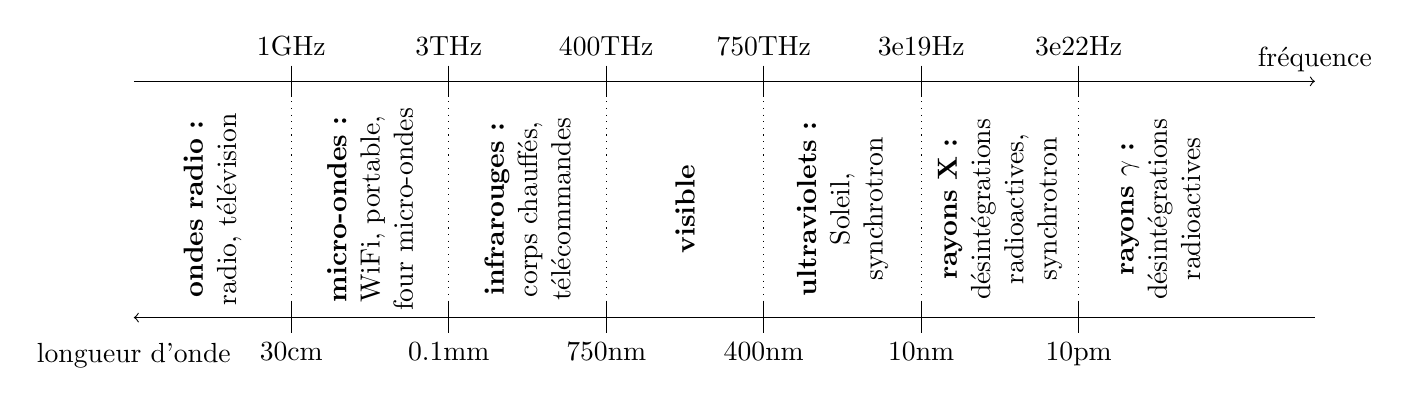
\begin{tikzpicture}[scale=1]
  %tikz ondes
\newcommand{\h}{0.2}
\draw[->] (0,0) -- (15,0) ;
\draw (15,0) node[anchor=south]{fréquence};
\def\H{-3}
\draw[->] (15,\H) -- (0,\H) ;
\draw (0,\H-0.2) node[anchor=north]{longueur d'onde};
 
\def\x{0}
%\draw (0,\h) -- (0,-\h) ;
%\draw (0,\h) node[anchor=south]{0};
%\draw (0,\H+\h) -- (0,\H-\h) ;
%\draw (0,\H-\h) node[anchor=north]{$\infty$};
%\draw[dotted] (\x,0) -- (\x,\H);

\draw (1,0) node[anchor=east,rotate=90,align=center,text width=3cm]{\textbf{ondes radio :}\\ radio, télévision}; 

\def\x{2}
\draw (\x,\h) -- (\x,-\h) ;
\draw (\x,\h) node[anchor=south]{\SI{1}{GHz}};
\draw (\x,\H+\h) -- (\x,\H-\h) ;
\draw (\x,\H-\h) node[anchor=north]{\SI{30}{cm}};
\draw[dotted] (\x,0) -- (\x,\H);

\draw (3,0) node[anchor=east,rotate=90,align=center,text width=3cm] {\textbf{micro-ondes :} \\ WiFi, portable, four micro-ondes}; 

\def\x{4}
\draw (\x,\h) -- (\x,-\h) ;
\draw (\x,\h) node[anchor=south]{\SI{3}{THz}};
\draw (\x,\H+\h) -- (\x,\H-\h) ;
\draw (\x,\H-\h) node[anchor=north]{\SI{0.1}{mm}};
\draw[dotted] (\x,0) -- (\x,\H);

\draw (5,0) node[anchor=east,rotate=90,align=center,text width=3cm]{\textbf{infrarouges :}\\corps chauffés, télécommandes};

\def\x{6}
\draw (\x,\h) -- (\x,-\h) ;
\draw (\x,\h) node[anchor=south]{\SI{400}{THz}};
\draw (\x,\H+\h) -- (\x,\H-\h) ;
\draw (\x,\H-\h) node[anchor=north]{\SI{750}{nm}};
\draw[dotted] (\x,0) -- (\x,\H);

\draw (7,0) node[anchor=east,rotate=90,align=center,text width=3cm]{\textbf{visible }};

\def\x{8}
\draw (\x,\h) -- (\x,-\h) ;
\draw (\x,\h) node[anchor=south]{\SI{750}{THz}};
\draw (\x,\H+\h) -- (\x,\H-\h) ;
\draw (\x,\H-\h) node[anchor=north]{\SI{400}{nm}};
\draw[dotted] (\x,0) -- (\x,\H);

\draw (9,0) node[anchor=east,rotate=90,align=center,text width=3cm]{\textbf{ultraviolets : } \\Soleil,\\ synchrotron};

\def\x{10}
\draw (\x,\h) -- (\x,-\h) ;
\draw (\x,\h) node[anchor=south]{\SI{3e19}{Hz}};
\draw (\x,\H+\h) -- (\x,\H-\h) ;
\draw (\x,\H-\h) node[anchor=north]{\SI{10}{nm}};
\draw[dotted] (\x,0) -- (\x,\H);

\draw (11,0) node[anchor=east,rotate=90,align=center,text width=3cm]{\textbf{rayons X :}\\ désintégrations radioactives, synchrotron};

\def\x{12}
\draw (\x,\h) -- (\x,-\h) ;
\draw (\x,\h) node[anchor=south]{\SI{3e22}{Hz}};
\draw (\x,\H+\h) -- (\x,\H-\h) ;
\draw (\x,\H-\h) node[anchor=north]{\SI{10}{pm}};
\draw[dotted] (\x,0) -- (\x,\H);

\draw (13,0) node[anchor=east,rotate=90,align=center,text width=3cm]{\vphantom{X}\textbf{rayons $\gamma$ :} \\ désintégrations radioactives};
\end{tikzpicture}
\item mécaniques : tremblements de terre
\item vagues, ... 
\end{itemize} 

\section{Ondes progressives}
On se limite à une propagation \emph{unidimensionnelle} dans un milieu \emph{linéaire} et \emph{non dispersif}.
Un milieu linéaire est un milieu dans lequel les amplitudes de deux ondes qui se superposent s'additionnent. 

\subsection{Milieu dispersif et non dispersif}%
\label{sub:milieu_dispersif_et_non_dispersif}
On dit qu'un milieu est \textbf{dispersif} lorsque la vitesse de propagation de l'onde dépend de sa fréquence (ou de sa longueur d'onde). Dans un milieu non dispersif, des ondes de fréquences différentes se propagent à la même vitesse.

Dans un milieu dispersif, les propriétés de propagation d'une onde dépendent de sa fréquence, le milieu pourra notamment séparer les différentes composantes sinusoïdales d'une onde. Par exemple, le verre est un milieu dispersif pour la lumière, ce qui permet de fabriquer un prisme qui décompose la lumière blanche. La propagation des vagues à la surface de l'eau est également dispersive.

Dans un milieu dispersif, une impulsion brève aura tendance à s'élargir au cours de sa propagation.

La propagation de la lumière dans le vide ainsi que celle du son dans l'air sont non dispersives.

\subsection{Propagation d'une onde}%
\label{sub:propagation_d_une_onde}



La vitesse de propagation de l'onde s'appelle la \emph{célérité} (notée $c$).

La grandeur physique perturbée lors de la propagation de l'onde est notée $y$, sa valeur dépend de la position $x$ dans le milieu et du temps $t$ auquel on la mesure donc $y=y(x,t)$, c'est une fonction de deux variables. 

On peut représenter l'allure de l'onde à un instant $t_1$ donnée c'est la \textbf{représentation spatiale} ou l'évolution de l'onde en un point $x$ donné, c'est la \textbf{représentation temporelle}.

\begin{center}
\begin{minipage}{0.5\linewidth}
\begin{center}
\begin{tikzpicture}[scale=0.8]
\draw[dotted, gray] (-1.5,-0.5) grid (6.5,2.5);
\draw[->] (-2,0) -- (7,0) node[below] {$x$(m)}; %axe horizontal
\newcommand\h{0.2}
\draw[->] (0,-1) -- (0,3) node[right] {y (propriété du milieu)}; %axe vertical
\foreach \x in {-1,0,1,2,3,4,5,6} {\draw (\x,0) --(\x,-\h) node[below,fill=white]{\x};}


%Forme à t=0s
\draw[color=coul1,line width=1pt] (-2,0.7) -- (1,0.7) -- (1,1.5) --(2,1.5) -- (2,0.2) -- (6,0.2);
\draw[color=coul1,line width=1pt] (5.2,2.2) -- (5.7,2.2) node[right,color=black,fill=white]{$t=\SI{0}{s}$};

%Forme à t=3s
\draw[color=coul2,line width=1pt] (-2,0.7) -- (3,0.7) -- (3,1.5) --(4,1.5) -- (4,0.2) -- (6,0.2);
\draw[color=coul2,line width=1pt] (5.2,1.6) -- (5.7,1.6) node[right,color=black,fill=white]{$t=\SI{2}{s}$};

%flèche c
\draw[->,line width=1pt] (2,2) -- (3,2) node[above]{$c=\SI{1}{m/s}$};

\draw (3,-1) node[below] {Représentation spatiale};
\end{tikzpicture}
\end{center}
\end{minipage}%
\begin{minipage}{0.5\linewidth}
\begin{center}
\begin{tikzpicture}[scale=0.8]
\draw[dotted, gray] (-1.5,-0.5) grid (6.5,2.5);
\draw[->] (-2,0) -- (7,0) node[below] {$t$(s)}; %axe horizontal
\newcommand\h{0.2}
\draw[->] (0,-1) -- (0,3) node[right] {y (propriété du milieu)}; %axe vertical
\foreach \x in {-1,0,1,2,3,4,5,6} {\draw (\x,0) --(\x,-\h) node[below,fill=white]{\x};}

%Forme à t=0s
\draw[color=coul1,line width=1pt] (-2,0.2) -- (0,0.2) -- (0,1.5) --(1,1.5) -- (1,0.5) -- (6,0.5);
\draw[color=coul1,line width=1pt] (5,2) -- (5.5,2) node[right,color=black]{$x=\SI{2}{m}$};

%Forme à t=3s
\draw[color=coul2,line width=1pt] (-2,0.2) -- (2,0.2) -- (2,1.5) --(3,1.5) -- (3,0.5) -- (6,0.5);
\draw[color=coul2,line width=1pt] (5,1.6) -- (5.5,1.6) node[right,color=black]{$x=\SI{4}{m}$};
 

%flèche c 
\draw (3,2) node[above]{$c=\SI{1}{m/s}$};

\draw (3,-1) node[below] {Représentation temporelle};
\end{tikzpicture}
\end{center}
\end{minipage}
\end{center}

\begin{application}
La foudre tombe à une distance $d$ d'un observateur, ce dernier mesure le temps $\Delta t$ qui sépare l'éclair du tonnerre et trouve $\Delta t=\SI{3}{s}$. Déterminer la distance $d$. 
\end{application}

Dans le cas général, une l'amplitude $y$ d'une onde varie dans le temps et l'espace, on représente alors l'onde par une fonction de plusieurs variables $y(x, t)$. 

Dans le cas d'une onde progressive se déplaçant dans le sens de $x$ croissants, on peut écrire :
\begin{center}
\newcommand\mytikzmark[2]{%
  \tikz[remember picture,baseline=(#1.base)]{\node(#1)[inner sep=0pt,outer sep=0pt]{#2};}%
}
\begin{tikzpicture}[remember picture]
\node(equation) at (0,0) {$\mytikzmark{y}{$y$}(x, t) = \mytikzmark{f}{$f$}(x-ct)$};
\node[below left, yshift = -0.5cm] (f1) at (y.south){Fonction de deux variables};
\node[below right, yshift = -0.5cm] (f2) at (f.south){Fonction d'une variable};
\draw[->] (f1.north) to[out=90, in=-90] ($(y.south)+(0,-0.1)$);
\draw[->] (f2.north) to[out=90, in=-90] ($(f.south)+(0,-0.1)$);
\end{tikzpicture}
\end{center}

Car l'onde reçue au point $M(x)$ au temps $t$ est la même que celle présente en $O$ au temps $t-\Delta t$. Où $\Delta t = \frac{x}{c}$ est le temps mis par l'onde pour se propager de $O$ à $M(x)$. Donc 

\begin{equation}
  y(x, t) = y(0, t-x/c) = f(x-ct)
\end{equation}.    

Dans ce cas, $\frac{x}{c}$ est le \emph{retard temporel} de l'onde au point d'abscisse $x$. 

De la même manière, une onde se propageant vers la gauche ($x$ décroissant) sera de la forme $y(x, t) = g(x+ct)$.  


\section{Ondes progressives sinusoïdales}
Une onde progressive sunusoïdale est une onde pour laquelle l'amplitude de la perturbation du milieu est donnée par : 
\begin{center}
  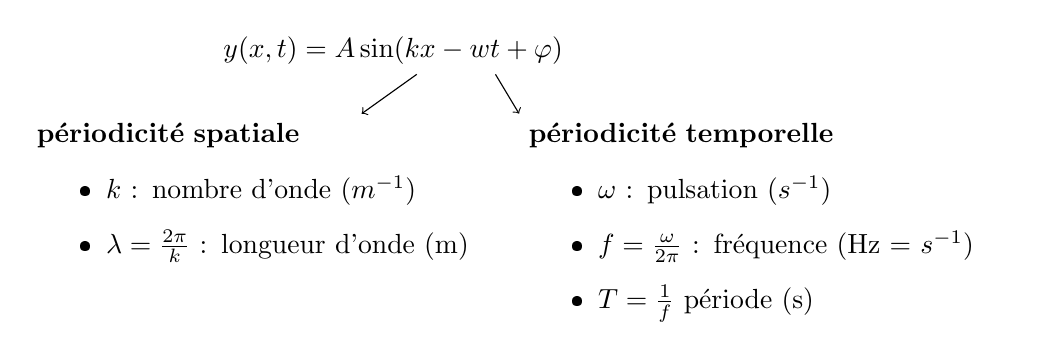
\begin{tikzpicture}
    \draw (4.4,0) node[anchor=south]{$y(x,t)=A\sin(kx-wt+\varphi)$}; 
    \draw[->] (4.7,0) -- (4,-0.5);
    \draw (6,-0.5) node[anchor=north east,text width=6cm]{
      \textbf{périodicité spatiale}
      \begin{itemize}
      \item $k$ : nombre d'onde ($\si{m^{-1}}$)
      \item $\lambda = \frac{2\pi}{k}$ : longueur d'onde (\si{m})
      \end{itemize}
    }; 
    \draw[->] (5.7,0) -- (6,-0.5);
    \draw (6,-0.5) node[anchor=north west,text width=6cm]{
      \textbf{périodicité temporelle}
      \begin{itemize}
      \item $\omega$ : pulsation ($\si{s^{-1}}$)
      \item $f = \frac{\omega}{2\pi}$ : fréquence (\si{Hz} = $\si{s^{-1}}$)
      \item $T = \frac{1}{f}$ période (\si{s})
      \end{itemize}
    };
  \end{tikzpicture}
\end{center}

La célérité de l'onde (dans ce cas, appelée \textbf{vitesse de phase})  est $c=\frac{\omega}{k}=\frac{2\pi f}{2\pi / \lambda} = f\lambda = \frac{\lambda}{T}$

\begin{minipage}{0.5\linewidth}
\begin{center}
\begin{tikzpicture}[scale=0.4]
  \draw[->] (-8,0) -- (8,0) node[right]{$x$};
  \draw[dotted](-8,3) -- (8,3);
  \draw[dotted](-8,-3) -- (8,-3);
  \draw[<->] (-7,0) -- (-7,3);
  \draw (-7,1.5) node[left] {$A$};
  \draw[->] (0,-3) -- (0,4.5) node[right]{$y(x,0)$};
  \draw[color=coul1,thick] plot[id=sinx,samples=100,domain=-8:8] function{3*sin(x)};
  \draw[<->] (-pi/2,-3.5) -- (3*pi/2,-3.5) ;
  \draw (pi/2,-3.5) node[below]{$\lambda$};
  \draw (0,-5) node[below] {\'Evolution spatiale};
\end{tikzpicture}
\end{center}
\end{minipage}%
\begin{minipage}{0.5\linewidth}
\begin{center}
\begin{tikzpicture}[scale=0.4]
  \draw[->] (-8,0) -- (8,0) node[right]{$t$};
  \draw[dotted](-8,3) -- (8,3);
  \draw[dotted](-8,-3) -- (8,-3);
  \draw[<->] (-7,0) -- (-7,3);
  \draw (-7,1.5) node[left] {$A$};
  \draw[->] (0,-3) -- (0,4.5) node[right]{$y(0,t)$};
  \draw[color=coul1,thick] plot[id=sinx,samples=100,domain=-8:8] function{3*sin(x)};
  \draw[<->] (-pi/2,-3.5) -- (3*pi/2,-3.5) ;
  \draw (pi/2,-3.5) node[below]{$T$};
  \draw (0,-5) node[below] {\'Evolution temporelle};
\end{tikzpicture}
\end{center}
\end{minipage}

La \emph{phase totale} de l'onde au point $x$ et au temps $t$ est $(kx-\omega t + \varphi)$. La phase à l'origine ($t=0$ et $x=0$)  est $\varphi$. La phase d'une onde se mesure en radians (rad).

\begin{application}
Calculer la longueur d'onde d'un son audible, la fréquence de la lumière visible
\end{application}

\section{Interférences entre deux ondes}
\subsection{Formule de Fresnel}%
\label{sub:formule_de_fresnel}


Dans un milieu \emph{linéaire} les perturbations de deux ondes qui se superposent s'additionnent.

Soient $S_1$ et $S_2$ deux sources d'ondes sinusoïdales de mêmes fréquence situées à deux positions différentes de l'axe $x$.
\begin{center}
\begin{tikzpicture}
\draw[->] (0,0) -- (10,0) node[right]{$x$};
\draw[fill=black] (1,0) circle (0.05) node[above]{$S_1$} node[below]{0};
\draw[fill=black] (3,0) circle (0.05) node[above]{$S_2$} node[below] {$d$};
\draw[fill=black] (8,0) circle (0.05) node[above]{$R$} node[below]{$x$};
\end{tikzpicture}
\end{center}

Au point $R$ d'abscisse $x$ on a :
\begin{itemize}
\item Onde émise par $S_1$ : $y_1(x,t) = A\cos(kx-\omega t)$
\item Onde émise par $S_2$ : $y_2(x,t) = B\cos(k(x-d)-\omega t) = B\sin(kx-\omega t-kd) = A\sin(kx-\omega t - \Delta\varphi)$
\end{itemize}

L'onde totale reçue en $R$ est alors 
\begin{align}
  y(x,t)=y_1(x,t) + y_2(x,t) &= A \cos(kx-\omega t) + B \cos(kx-\omega t - kd) \\&= A \cos(kx-\omega t) + B \cos(kx-\omega t - \Delta\varphi)
\end{align} 
La grandeur $kd=\Delta\varphi$ est appelée \emph{déphasage} entre les deux ondes.

Ce qui nous intéresse particulièrement, c'est l'amplitude des oscillations de $y(x, t)$. Pour déterminer cette amplitude, nous allons passer par la notation complexe. On a 
\begin{equation}
  \ul{y}(x, t) = Ae^{i(kx-\omega t)} + Be^{i(kx-\omega t - \Delta\varphi)} = e^{i(kx-\omega t - \frac{\Delta\varphi}{2})}\left( Ae^{\frac{i\Delta\varphi}{2}} + Be^{-i\frac{\Delta\varphi}{2}} \right) 
\end{equation}

L'amplitude $Y$ de $y(x, t)$ est
\begin{align}
  Y = |\ul{y}(x, t)|
  &= \left| Ae^{\frac{i\Delta\varphi}{2}} + Be^{-i\frac{\Delta\varphi}{2}} \right| = 
  \left| 
    (A+B)\cos\left(\frac{\Delta\varphi}{2}\right) + 
   i(A-B) \sin\left(\frac{\Delta\varphi}{2}\right) 
  \right|  \\
  &= \sqrt{(A+B)^2\cos^2\left(\frac{\Delta\varphi}{2}\right) + 
           (A-B)^2\sin^2\left(\frac{\Delta\varphi}{2}\right) }\\
  &= \sqrt{A^2 + B^2 + 2AB\cos\left(\Delta\varphi \right) }
\end{align}

On obtient alors la \textbf{formule de Fresnel}, qui donne l'amplitude $Y$  resultant de la superposition de deux ondes de même fréquence et d'amplitudes $A$ et $B$ déphasées de $\Delta\varphi$  :
\begin{eqencadre}
  Y = \sqrt{A^2 + B^2 + 2AB\cos(\Delta\varphi)}
  \label{eq:fresnel}
\end{eqencadre}

Le terme $2AB\cos(\Delta\varphi)$ est le \textbf{terme d'interférence}.   

%On peut également utiliser la \textit{représentation de Fresnel} pour calculer la somme de deux fonctions trigonométrique. On représente une onde d'amplitude $y_1(x, t) = A\sin(\omega t + \varphi)$ par un vecteur de norme $A$ formant un angle $\varphi$ avec l'horizontale. L'amplitude de l'onde resultante de la superposition de deux ondes déphasées sera la norme de la somme des vecteurs représentant ces deux ondes. La superposition des deux ondes précédentes est représentée sur le schéma ci-dessous.

%\begin{center}
%\begin{tikzpicture}
%\draw[-latex] (0,0) -- (6,0) node[right]{$x$};
%\draw[thick, coul1, -latex] (0,0) -- ++(3,0) node[midway, below]{$A$}; 
%\draw[thick, coul2, -latex] (3,0) -- ++(40:3) node[midway, below right]{$A$} coordinate (B); 
%\draw (3.8,0) arc(0:40:0.8) node[midway, right]{$\varphi$}; 
%\draw[thick, -latex] (0,0) -- (B) node[midway, sloped, above] {$2A\cos\left( \frac{\Delta\varphi}{2} \right) $ };
%\end{tikzpicture}
%\end{center}

%Dans ce cas précis, la représentation de Fresnel ne simplifie pas considérablement le calcul, mais c'est un outil qui peut être utile, notamment lorsque les amplitudes des ondes qui interfèrent sont différentes.

\begin{itemize}
  \item Si $\Delta\varphi=2n\pi \Leftrightarrow d=n\lambda$, le terme d'interférence est maximum (positif), l'amplitude résultante est maximale : \emph{Interférences constructives}
  \item  Si $\Delta\varphi=(2n+1)\pi \Leftrightarrow d=\left(n+\frac{1}{2}\right)\lambda$, le terme d'interférence est minimum (négatif), l'amplitude résultante est minimale : \emph{Interférences destructives}
\end{itemize}

Ci-dessous on représente la situation des interférences constructives et destructives dans le cas où les amplitudes des deux ondes qui interfèrent sont identiques. Dans ce cas particulier, lorsque les interférences sont destructives, l'amplitude resultante est nulle.

%Interprétation graphique
\begin{minipage}{0.5\linewidth}
  \begin{center}
    \begin{tikzpicture}[scale=0.3]
        %tikz ondes
        \draw[->] (-3*pi,0) -- (8,0) node[right]{$x$}; 
        \draw[->] (0,-3) -- (0,4.5) node[right]{$y(x,0)$};
        \draw[red,thick] plot[samples=100,domain=-3*pi:8] (\x,{3*sin(\x r)});
        \draw[blue,thick] plot[samples=100,domain=-3*pi+0.2+2*pi:8] (\x, {3*sin((\x-0.2) r)});
        \draw[color=coul1,fill=coul1] (-3*pi,0) circle (0.1) node[above]{$S_1$};
        \draw[color=coul2,fill=coul2] (-pi+0.2,0) circle (0.1) node[above]{$S_2$};
        \draw[<->] (-3*pi,-3.5) -- (-1*pi,-3.5) ;
        \draw[dotted] (-3*pi,0) -- (-3*pi,-3.5) ;
        \draw[dotted] (-pi,0) -- (-pi,-3.5) ;  
        \draw (-1.5*pi,-3.5) node[below]{$d=\lambda \Leftrightarrow \Delta\varphi=2\pi$};
        \draw (0,-6) node[below] {interférences constructives $\Delta\varphi = 2n\pi$};
    \end{tikzpicture}
  \end{center}
\end{minipage}%
\begin{minipage}{0.5\linewidth}
\begin{center}
    \begin{tikzpicture}[scale=0.3]
        %tikz ondes
        \draw[->] (-3*pi,0) -- (8,0) node[right]{$x$}; 
        \draw[->] (0,-3) -- (0,4.5) node[right]{$y(x,0)$};
        \draw[color=coul1,thick] plot[samples=100,domain=-3*pi:8] (\x, {3*sin(\x r)});
        \draw[color=coul2,thick] plot[samples=100,domain=-3*pi+pi:8] (\x, {3*sin((\x-pi) r)});
        \draw[color=coul1,fill=coul1] (-3*pi,0) circle (0.1) node[above]{$S_1$};
        \draw[color=coul2,fill=coul2] (-2*pi,0) circle (0.1) node[above]{$S_2$};
        \draw[<->] (-3*pi,-3.5) -- (-2*pi,-3.5) ;
        \draw[dotted] (-3*pi,0) -- (-3*pi,-3.5) ;
        \draw[dotted] (-2*pi,0) -- (-2*pi,-3.5) ;
        \draw (-2.5*pi,-3.5) node[below]{$d=\lambda/2 \Leftrightarrow \Delta\varphi=\pi$};
        \draw (0,-6) node[below] {interférences destructives $\Delta\varphi = (2n+1)\pi$};
    \end{tikzpicture}
  \end{center}
\end{minipage}

\subsection{Interférences lumineuses}%
\label{sub:interferences_lumineuses}
Une onde lumineuse est une onde électromagnétique, c'est à dire qu'elle est due aux oscillations des champs électrique et magnétique. On peut montrer qu'une onde électromagnétique est entièrement déterminée par la donnée de son champ électrique elle sera donc représentée par son vecteur champ électrique $\vv{E}(\vv{r}, t)$. 

Lorsque deux ondes lumineuses se superposent, les vecteurs champ électrique s'additionnent. Il faut faire la somme vectorielle des champs électriques.

La direction du champ électrique est la \textbf{polarisation} de la lumière. Dans cette partie, nous considérerons que la polarisation de la lumière est toujours suivant une direction $\vv{u}$ fixe, de telle sorte que nous puissions écrire le champ électrique comme
\begin{equation}
  \vv{E}(\vv{r}, t) = E(\vv{r}, t)\vv{u}
\end{equation}

Cela nous permet de représenter une onde lumineuse uniquement par la projection $\vv{E}(\vv{r}, t)$ de son champ électrique selon le vecteur $\vv{u}$. On passe donc d'une représentation vectorielle à une représentation scalaire de la lumière.  

Une source ponctuelle monochromatique émet une onde dont l'amplitude à une distance $r$ de la source est
\begin{equation}
  s(r, t) = \frac{A}{r}\cos(kr-\omega t),
\end{equation}

avec $k = n\frac{\omega}{c} = n\frac{2\pi}{\lambda_0}$, où $\lambda_0$ est la longueur d'onde dans le vide de l'onde. 

Le déphasage subi par une onde se propageant de $S$ à $M$ parcourant une distance $r$ dans un milieu d'indice $n$ sera $\varphi = kr =  \frac{2\pi nr}{\lambda_0}$. On note alors $[SM] = nr$, cette grandeur est appelée le \textbf{chemin optique} parcouru par la lumière. C'est la distance parcourue multipliée par l'indice du milieu.

\begin{loi}{Déphasage entre deux ondes lumineuses}
  Le déphasage entre deux ondes lumineuses émises par une source $S$ arrivant en un point $M$ parcourant des chemins optiques $[SM]_1$ et $[SM]_2$ est donné par
  \begin{equation}
    \Delta\varphi = \frac{2\pi}{\lambda_0}\left( [SM]_2-[SM]_1 \right) = \frac{2\pi}{\lambda_0}\delta
  \end{equation}
  La grandeur $\delta$ est appelée \textit{différence de marche} entre les deux ondes, c'est la différence de chemin optique entre les deux ondes. 
\end{loi}

Nous allons appliquer étudier un exemple important d'interférences lumineuses : \textbf{l'expérience des trous d'Young}. 

Dans cette expérience, on éclaire deux ouvertures espacées d'une distance $a$  avec une source ponctuelle monochromatique et on observe l'intensité lumineuse reçue sur un écran éloigné (à une distance $D$ des ouvertures).
\begin{center}
  \begin{tikzpicture}
    %tikz ondes
            \draw[->] (10, -4) -- (10, 4) node[right]{$x$} ;
            \draw[->] (4, 0) -- (12, 0) node[right]{$z$}; 
    \fill (0,0) coordinate (S) circle(2pt) ;
    \coordinate (A1) at (4.05, 0.95);
    \coordinate (A2) at (4.05, -0.95);
\node[below] at (0,-2pt) {$S$ };  
\fill[gray] (4, 3) rectangle (4.1, 1)
              (4, 0.9) rectangle (4.1, -0.9)
              (4, -1) rectangle (4.1, -3);

            \fill (10,1) coordinate(M) circle(2pt) ;
            \node[right] at (10.1,1) {$M(x)$ };  
            \draw[<->] (4.1, -3) -- (10, -3) node[midway, below]{$D$}; 
            \draw[<->] (3.8, -0.90) -- (3.8, 0.90) node[midway, left]{$a$}; 
            \node[above right] at (4.1, 1) {$A_1$}; 
            \node[below right] at (4.1, -1) {$A_2$}; 
            \draw (S) -- (A1) -- (M);
            \draw (S) -- (A2) -- (M);
            %\draw (10, 0) -- (10.2, 0) node[right]{$0$}; 
  \end{tikzpicture}
  \captionof{figure}{Schématisation du dispositif des trous d'Young.}
\end{center}
Calculons la différence de marche $\delta$ entre les deux ondes arrivant en $M$ :
\begin{align}
  \delta &= [SA_2M] - [SA_1M] = [SA_2] + [A_2M] - ([SA_1] + [A_1M]) = [A_2M] - [A_1M] \\
         &= A_2M - A_1M
\end{align}
On considère que l'expérience est menée dans l'air d'indice $n=1$. L'application du théorème de Pythagore donne:
\begin{equation}
  A_1M = \sqrt{D^2 + \left(x-\frac{a}{2}\right)^2} \quad \text{et} \quad A_2M = \sqrt{D^2+ \left(x+\frac{a}{2}\right)^2}
\end{equation}

Nous allons nous placer dans la situation où les interférences sont observées sur un écran placé \textit{loin} des fentes, . Plus précisément, on considère que
\begin{equation}
  D \gg x \quad \text{et} \quad D \gg a
\end{equation}
Dans ces conditions, on peut écrire 
\begin{equation}
  A_1M  = D \sqrt{1+\left( \frac{2x-a}{2D} \right)^2 } \quad \text{et} \quad A_2M  = D \sqrt{1+\left( \frac{2x+a}{2D} \right)^2 }
\end{equation}
Comme $\left( \frac{2x-a}{2D} \right)^2 \ll 1$ et $\left( \frac{2x+a}{2D} \right)^2\ll 1$ On peut faire un développement limité à l'ordre 1 de la racine en écrivant que $\sqrt{1+\varepsilon} \approx 1+\frac{1}{2}\varepsilon$ et on obtient
\begin{equation}
  A_1M = D\left(1+\frac{1}{2}\left( \frac{2x-a}{2D} \right)^2\right) \quad \text{et} \quad A_2M = D\left(1+\frac{1}{2}\left( \frac{2x+a}{2D} \right)^2\right)
\end{equation}
La différence de marche entre les deux ondes arrivant en $M$ devient alors :
\begin{equation}
  \delta = A_2M - A_1M = D + \frac{1}{8D} \left( 4x^2 + 4ax + a^2 \right) -D -\frac{1}{8D} \left( 4x^2 - 4ax + a^2 \right) = \frac{ax}{D}
\end{equation}
On trouve donc finalement
\begin{eqencadre}
  \delta = \frac{ax}{D}
\end{eqencadre}

On suppose que les deux ondes qui interfèrent en $M$ ont la même amplitude $E$.  Dans ce cas, la formule de Fresnel \eqref{eq:fresnel} donne l'amplitude de l'onde en fonction de $x$ :
\begin{equation}
  S(x) = \sqrt{2}E \sqrt{1 + \cos\left( \frac{2\pi ax}{\lambda_0D} \right) }
\end{equation}

Or, l'intensité lumineuse, qui correspond à la puissance transportée par l'onde lumineuse, est proportionelle au carré de l'amplitude du champ électrique, on aura donc l'intensité :
\begin{eqencadre}
  I(x) = 2I_0\left(1+\cos\left( \frac{2\pi ax}{\lambda_0D}\right) \right)
\end{eqencadre}
où $I_0$ est l'intensité lumineuse produite sur l'écran lorsqu'un seul des deux trous est ouvert. On observer sur l'écran une alternance de franges sombres et brillantes.
 \usetikzlibrary{calc}
 \begin{center}
 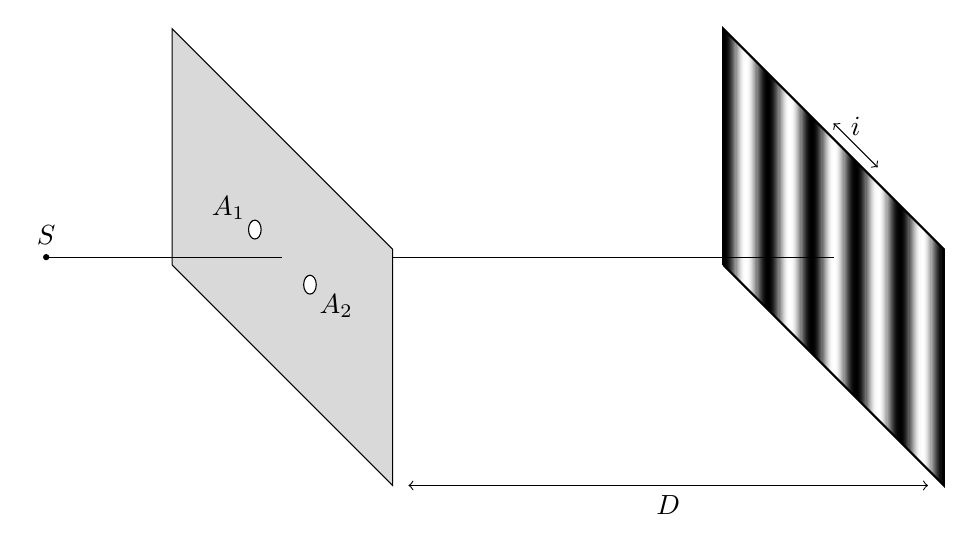
\begin{tikzpicture}[z={(0.7, -0.7)}]

    %tikz ondes
% ---- Customizable section
\def\numsamples{200}   % The greater, the thinner each sample
\def\numcycles{5}      % Number of "white bars" in the result
\def\totalwidth{4}    % Width (in cm) of the resulting box
% ---- End of customizable section

\pgfmathsetmacro{\samplewidth}{\totalwidth/\numsamples}
\pgfmathsetmacro{\frequency}{360/\numsamples*\numcycles}
\foreach \i in {0,...,\numsamples} {
  \pgfmathsetmacro{\shade}{50+50*sin(\i*\frequency+90)}
\fill[draw=none, fill=black!\shade!white] (10, 0, {\i*\samplewidth-\totalwidth/2}) rectangle +(0, 3, \samplewidth*1.1);
}
\draw[thick] (10,0, -\totalwidth/2) -- ++(0, 3, 0) -- ++(0, 0, \totalwidth) -- ++(0, -3, 0) -- ++(0, 0, -\totalwidth);
\draw (3,1.5,0) -- ++(7, 0,0);
\draw[fill=gray!30] (3, 0, -2) -- ++(0, 3, 0) -- ++(0, 0, 4) -- ++(0, -3, 0) -- ++(0, 0, -4);
\draw (0,1.5,0) -- ++(3, 0,0);
\fill[white, draw=black] (3, 1.5, 0.5) circle(0.8mm and 1.2mm) node[below right, black]{$A_2$} ;
\fill[white, draw=black] (3, 1.5, -0.5) circle(0.8mm and 1.2mm) node[above left, black]{$A_1$};
\fill (0,1.5) circle (0.4mm) node[above, yshift=0.4mm] {$S$ };
\draw[<->] (3.2, 0, 2) -- (9.8, 0, 2) node[midway, below]{$D$}; 
\draw[<->] (10, 3.2, 0) -- (10, 3.2, 0.8) node[midway, above]{$i$};
\end{tikzpicture}
\captionof{figure}{Allure de l'éclairement de l'écran placé à grande distance des trous d'Young}
\end{center}

L'\textbf{interfrange} $i$ correspond à la distance séparant deux franges lumineuses. La première frange lumineuse se trouvant au centre de l'écran ($x=0$), la seconde se trouve à une abscisse $i$ telle que 
\begin{equation}
  \frac{2\pi ai}{\lambda_0D} = 2\pi
\end{equation} 
soit
\begin{eqencadre}
  i = \frac{\lambda_0D}{a} 
\end{eqencadre}

\end{document}

 %%% Local Variables: 
 %%% mode: latex
 %%% LaTeX-command: "latex -shell-escape"
 %%% End:
